\chapter{Functional methods in Quantum Field Theory}
\blindtext
\section{Generating Functionals and Correlation Functions}
We consider a theory setting of $N$ scalar fields $\varphi_a(x), a \in \{1,\dots,N\}$ in $d$-dimensional Euclidean space. The corresponding partition sum in presence of sources $J_a(x)$ reads
\begin{align}
	Z[J] =  \int \D\varphi \operatorname{e}^{-\S + J\cdot\varphi}.
\end{align}
The information content of the partition sum results mainly from the classical action functional $\S$, which determines the classical field equations
\begin{align}
	\frac{\delta \mathcal{S}}{\delta\varphi(x)} = 0.
\end{align}
\textbf{Notation:} The scalar product sums over field components and integrates over all space \dots
\begin{align}
	J\cdot\varphi = \int_x J_a(x) \ \varphi_a(x) = \int_p \tilde{J}_a(p) \ \tilde{\varphi}_a(p)
\end{align}
with
\begin{align}
\int_x = \int_{\mathbb{R}^d} \dd^d x \qquad \text{and} \qquad \int_p = \int_{\mathbb{R}^d} \frac{\dd^d p}{(2\pi)^d}	
\end{align}

Mean field description:
\begin{align}
	\phi := \cf{\varphi} = \eval{\frac{1}{Z}\frac{\delta Z}{\delta J}}_{J=0} = \int \D\varphi \ \varphi \ \operatorname{e}^{-\S + J\cdot\varphi}  
\end{align}

Higher correlations:
\begin{align}
\cf{\varphi_1 \cdots \varphi_n} := \cf{\varphi^n} = \frac{1}{Z}\frac{\delta^n Z}{\delta^n J} = \int \D\varphi \ \overbrace{\varphi_1 \cdots \varphi_n}^{:= \ \varphi^n} \ \operatorname{e}^{-\S + J\cdot\varphi}  
\end{align}

We obtain the Schwinger functional by taking the logarithm:
\begin{align}
	W[J] = \ln Z[J]
\end{align}

For the special case of $n=2$ the correlation function yields the connected 2-point function which is also known as the propagator $G_{ab}(x, y)$ correlating the field $\varphi_a$ at spacetime point $x$ with the field $\varphi_b$ at $y$.
\begin{align}
	G_{ab}(x, y) &= \frac{\delta^2W[J]}{\delta J_a(x)\delta J_b(y)} = \frac{\delta}{\delta J_a(x)}\left(\frac{1}{Z}\frac{\delta Z}{\delta J_b(y)}\right) \nonumber \\
				&= \frac{1}{Z}\left(\frac{\delta^2Z}{\delta J_a(x)\delta J_b(y)}\right) - \frac{1}{Z^2}\left(\frac{\delta Z}{\delta J_a(x)}\right)\left(\frac{\delta Z}{\delta J_b(y)}\right)\\
				&= \cf{\varphi_a(x)\varphi_b(y)} - \phi_a(x)\phi_b(y) = \cf{\varphi_a(x)\varphi_b(y)}_{\text{c}}	\nonumber	
\end{align}

The Effective Action:\\

The effective action can be obtained by performing a Legendre transform of the Schwinger funtional, i.\,e.:
\begin{align}
\Gamma[\phi] = \underset{J}{\operatorname{sup}}\left\{ \int\limits_x J(x)\phi(x) - \W \right\} = \int\limits_x J_{\text{sub}}(x)\phi(x) - \mathcal{W}[J_{\text{sub}}]
\end{align}

Quantum equation of motion:
\begin{align}
\frac{\delta\Gamma[\phi]}{\delta\phi(x)} = J(x)	
\end{align}

Dyson-Schwinger equation:
\begin{align}
\frac{\delta\Gamma[\phi]}{\delta\phi(x)} = \frac{\delta\mathcal{S}}{\delta\varphi(x)} \left[\varphi = G \cdot \frac{\delta}{\delta\phi} + \phi \right]
\end{align}

\section{The Functional Renormalization Group}
\begin{itemize}
	\item Kadanoff Block-Spin model 
	\item maybe visualization of Ising model + phase transitions
\end{itemize}

\begin{figure}[H]
\centering
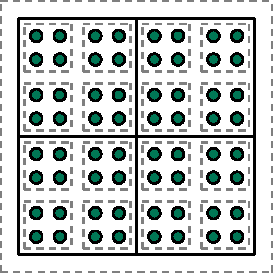
\includegraphics{figs/TikZ/block_spin_model}
\caption[Visualization of the Kadanoff Block-Spin model.]{Visualization of the Kadanoff Block-Spin model.\footnotemark}
\label{fig:kadanoff}
\end{figure}
\footnotetext{This visualization is inspired by an image provided in the \href{https://arxiv.org/pdf/cond-mat/0207340.pdf}{PhD thesis} of J.R. Laguna.}
\blindtext

\section{Renormalization Group Consistency}
This section is mainly based on \cite{BraunLeonhardtPawlowski2018}.

Cutoff independence of the full quantum effective action:
\begin{align}
	\Lambda\frac{\dd\Gamma}{\dd\Lambda} = 0
\end{align}

Full effective action in a generic representation:
\begin{align}
	\Gamma[\phi] = \D_{\Lambda}[\phi] + \Gamma_{\Lambda}[\phi]
\end{align}

Formal discussion:
\begin{align}
\Gammak[\phi] = \Gamma_{\Lambda}[\phi] + \int\limits_{\Lambda}^k \frac{\dd k'}{k'} \mathcal{F}_{k'}[\phi]
\end{align}
 
 
\section{Flow Equations for Generating Functionals}
We introduce the RG time scale $t$:
\begin{align}
	\partial_t = \frac{\partial}{\partial\ln(k/\Lambda)} = \frac{k}{\Lambda}\frac{\partial}{\partial(k/\Lambda)} = k \partial_k
\end{align}

\blindtext

\begin{align}
	\partial_t\Gammak[\phi] &= \frac{1}{2}\tr{\frac{1}{\Gammak^{(2)}[\phi] + R_k} \partial_t R_k} \nonumber \\ \phantom{.}  \\
							&= \frac{1}{2}\int\limits_p \frac{1}{\Gammak^{(2)}[\phi] + R_k}(p, -p) \ \partial_t R_k(p^2) \nonumber
\end{align}
This translates directly into the following diagrammic representation:

\begin{figure}[H]
\centering
\begin{gather}
\begin{aligned}
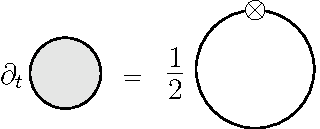
\includegraphics{figs/TikZ/wetterich_equation} 
\end{aligned}
\end{gather}
\end{figure}
where $\otimes = \partial_t R_k$ represents the insertion of the respective regulator. \\


\blindtext

\begin{figure}[H]
\centering
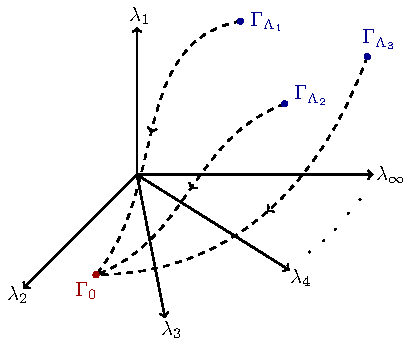
\includegraphics{figs/TikZ/regulator_dependence}
\caption[Flow of $\Gamma_k$ through infinite-dimensional theory space for different regulators.]{Flow of $\Gamma_k$ through infinite-dimensional theory space for different regulators, inspired by \cite{Riebesell2017}}	
\end{figure}